\subsection{Resumo}

\begin{table}[h!]
\centering
\begin{tabular}{ |c|c|c|c|c|  }
\hline
\rowcolor{lightgray}
Algoritmo & Max & Min & Média & Desvio Padrão \\
\hline
Hill-Climbing & 11773.256 & 9209.255 & 10531.702 & 919.177 \\
\hline
Hill-Climbing com restart & 9316.101 & 7665.887 & 8626.72 & 539.401 \\
\hline
Simulated Annealing & 11707.327 & 7730.449 & 10000.987 & 1089.323 \\
\hline
Genetic Algorithm & 17478.514 & 15008.897 & 16138.323 & 883.279 \\
\hline

\end{tabular}
\caption{Tabela com dados consolidados dos algoritmos}
\end{table}

\begin{figure}[H]
\centering
  \begin{minipage}[b]{0.48\textwidth}
    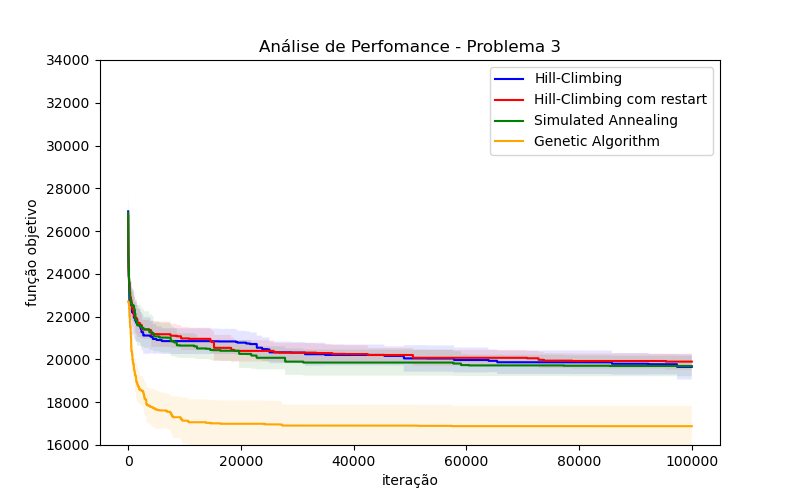
\includegraphics[width=88mm]{imagens/otima/problema-3-performance-algoritmos-best.png}
    \caption{Dados da execução da função objetivo durante as 10 iterações por melhor valor.
    \label{fig:problema-3-performance-algoritmos-best}}
  \end{minipage}
  \hfill
  \begin{minipage}[b]{0.48\textwidth}
    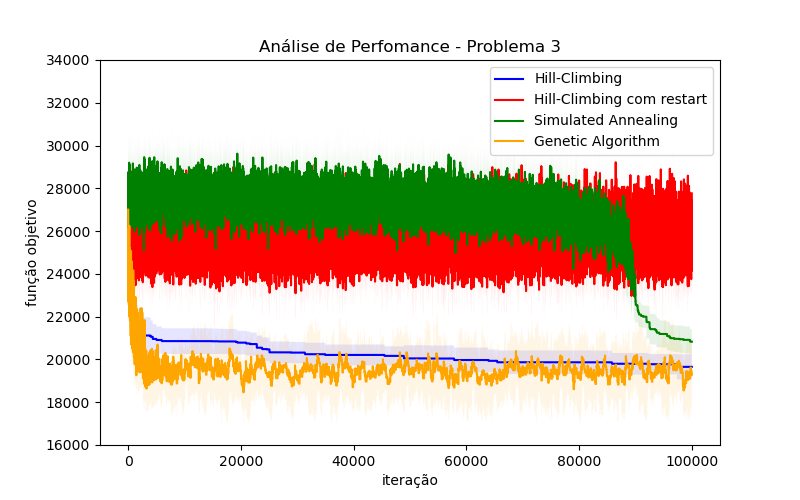
\includegraphics[width=88mm]{imagens/otima/problema-3-performance-algoritmos-value.png}
    \caption{Dados da execução da função objetivo durante as 10 iterações por valor atual.
    \label{fig:problema-3-performance-algoritmos-value}}
  \end{minipage}
\end{figure}